\documentclass[11pt]{article}
\usepackage{float}
% NOTE: Add in the relevant information to the commands below; or, if you'll be using the same information frequently, add these commands at the top of paolo-pset.tex file. 
\newcommand{\name}{Agustín Esteva}
\newcommand{\email}{aesteva@uchicago.edu}
\newcommand{\classnum}{23500}
\newcommand{\subject}{Markov Chains, Martingales, and Brownian Motion}
\newcommand{\instructors}{Stephen Yearwood}
\newcommand{\assignment}{Problem Set 1}
\newcommand{\semester}{Spring 2025}
\newcommand{\duedate}{04/04/2025}
\newcommand{\bA}{\mathbf{A}}
\newcommand{\bB}{\mathbf{B}}
\newcommand{\bC}{\mathbf{C}}
\newcommand{\bD}{\mathbf{D}}
\newcommand{\bE}{\mathbf{E}}
\newcommand{\bF}{\mathbf{F}}
\newcommand{\bG}{\mathbf{G}}
\newcommand{\bH}{\mathbf{H}}
\newcommand{\bI}{\mathbf{I}}
\newcommand{\bJ}{\mathbf{J}}
\newcommand{\bK}{\mathbf{K}}
\newcommand{\bL}{\mathbf{L}}
\newcommand{\bM}{\mathbf{M}}
\newcommand{\bN}{\mathbf{N}}
\newcommand{\bO}{\mathbf{O}}
\newcommand{\bP}{\mathbf{P}}
\newcommand{\bQ}{\mathbf{Q}}
\newcommand{\bR}{\mathbf{R}}
\newcommand{\bS}{\mathbf{S}}
\newcommand{\bT}{\mathbf{T}}
\newcommand{\bU}{\mathbf{U}}
\newcommand{\bV}{\mathbf{V}}
\newcommand{\bW}{\mathbf{W}}
\newcommand{\bX}{\mathbf{X}}
\newcommand{\bY}{\mathbf{Y}}
\newcommand{\bZ}{\mathbf{Z}}
\newcommand{\Vol}{\text{Vol}}

%% blackboard bold math capitals
\newcommand{\bbA}{\mathbb{A}}
\newcommand{\bbB}{\mathbb{B}}
\newcommand{\bbC}{\mathbb{C}}
\newcommand{\bbD}{\mathbb{D}}
\newcommand{\bbE}{\mathbb{E}}
\newcommand{\bbF}{\mathbb{F}}
\newcommand{\bbG}{\mathbb{G}}
\newcommand{\bbH}{\mathbb{H}}
\newcommand{\bbI}{\mathbb{I}}
\newcommand{\bbJ}{\mathbb{J}}
\newcommand{\bbK}{\mathbb{K}}
\newcommand{\bbL}{\mathbb{L}}
\newcommand{\bbM}{\mathbb{M}}
\newcommand{\bbN}{\mathbb{N}}
\newcommand{\bbO}{\mathbb{O}}
\newcommand{\bbP}{\mathbb{P}}
\newcommand{\bbQ}{\mathbb{Q}}
\newcommand{\bbR}{\mathbb{R}}
\newcommand{\bbS}{\mathbb{S}}
\newcommand{\bbT}{\mathbb{T}}
\newcommand{\bbU}{\mathbb{U}}
\newcommand{\bbV}{\mathbb{V}}
\newcommand{\bbW}{\mathbb{W}}
\newcommand{\bbX}{\mathbb{X}}
\newcommand{\bbY}{\mathbb{Y}}
\newcommand{\bbZ}{\mathbb{Z}}

%% script math capitals
\newcommand{\sA}{\mathscr{A}}
\newcommand{\sB}{\mathscr{B}}
\newcommand{\sC}{\mathscr{C}}
\newcommand{\sD}{\mathscr{D}}
\newcommand{\sE}{\mathscr{E}}
\newcommand{\sF}{\mathscr{F}}
\newcommand{\sG}{\mathscr{G}}
\newcommand{\sH}{\mathscr{H}}
\newcommand{\sI}{\mathscr{I}}
\newcommand{\sJ}{\mathscr{J}}
\newcommand{\sK}{\mathscr{K}}
\newcommand{\sL}{\mathscr{L}}
\newcommand{\sM}{\mathscr{M}}
\newcommand{\sN}{\mathscr{N}}
\newcommand{\sO}{\mathscr{O}}
\newcommand{\sP}{\mathscr{P}}
\newcommand{\sQ}{\mathscr{Q}}
\newcommand{\sR}{\mathscr{R}}
\newcommand{\sS}{\mathscr{S}}
\newcommand{\sT}{\mathscr{T}}
\newcommand{\sU}{\mathscr{U}}
\newcommand{\sV}{\mathscr{V}}
\newcommand{\sW}{\mathscr{W}}
\newcommand{\sX}{\mathscr{X}}
\newcommand{\sY}{\mathscr{Y}}
\newcommand{\sZ}{\mathscr{Z}}


\renewcommand{\emptyset}{\O}

\newcommand{\abs}[1]{\lvert #1 \rvert}
\newcommand{\norm}[1]{\lVert #1 \rVert}
\newcommand{\sm}{\setminus}


\newcommand{\sarr}{\rightarrow}
\newcommand{\arr}{\longrightarrow}

% NOTE: Defining collaborators is optional; to not list collaborators, comment out the line below.
%\newcommand{\collaborators}{Alyssa P. Hacker (\texttt{aphacker}), Ben Bitdiddle (\texttt{bitdiddle})}

% Copyright 2021 Paolo Adajar (padajar.com, paoloadajar@mit.edu)
% 
% Permission is hereby granted, free of charge, to any person obtaining a copy of this software and associated documentation files (the "Software"), to deal in the Software without restriction, including without limitation the rights to use, copy, modify, merge, publish, distribute, sublicense, and/or sell copies of the Software, and to permit persons to whom the Software is furnished to do so, subject to the following conditions:
%
% The above copyright notice and this permission notice shall be included in all copies or substantial portions of the Software.
% 
% THE SOFTWARE IS PROVIDED "AS IS", WITHOUT WARRANTY OF ANY KIND, EXPRESS OR IMPLIED, INCLUDING BUT NOT LIMITED TO THE WARRANTIES OF MERCHANTABILITY, FITNESS FOR A PARTICULAR PURPOSE AND NONINFRINGEMENT. IN NO EVENT SHALL THE AUTHORS OR COPYRIGHT HOLDERS BE LIABLE FOR ANY CLAIM, DAMAGES OR OTHER LIABILITY, WHETHER IN AN ACTION OF CONTRACT, TORT OR OTHERWISE, ARISING FROM, OUT OF OR IN CONNECTION WITH THE SOFTWARE OR THE USE OR OTHER DEALINGS IN THE SOFTWARE.

\usepackage{fullpage}
\usepackage{enumitem}
\usepackage{amsfonts, amssymb, amsmath,amsthm}
\usepackage{mathtools}
\usepackage[pdftex, pdfauthor={\name}, pdftitle={\classnum~\assignment}]{hyperref}
\usepackage[dvipsnames]{xcolor}
\usepackage{bbm}
\usepackage{graphicx}
\usepackage{mathrsfs}
\usepackage{pdfpages}
\usepackage{tabularx}
\usepackage{pdflscape}
\usepackage{makecell}
\usepackage{booktabs}
\usepackage{natbib}
\usepackage{caption}
\usepackage{subcaption}
\usepackage{physics}
\usepackage[many]{tcolorbox}
\usepackage{version}
\usepackage{ifthen}
\usepackage{cancel}
\usepackage{listings}
\usepackage{courier}

\usepackage{tikz}
\usepackage{istgame}

\hypersetup{
	colorlinks=true,
	linkcolor=blue,
	filecolor=magenta,
	urlcolor=blue,
}

\setlength{\parindent}{0mm}
\setlength{\parskip}{2mm}

\setlist[enumerate]{label=({\alph*})}
\setlist[enumerate, 2]{label=({\roman*})}

\allowdisplaybreaks[1]

\newcommand{\psetheader}{
	\ifthenelse{\isundefined{\collaborators}}{
		\begin{center}
			{\setlength{\parindent}{0cm} \setlength{\parskip}{0mm}
				
				{\textbf{\classnum~\semester:~\assignment} \hfill \name}
				
				\subject \hfill \href{mailto:\email}{\tt \email}
				
				Instructor(s):~\instructors \hfill Due Date:~\duedate	
				
				\hrulefill}
		\end{center}
	}{
		\begin{center}
			{\setlength{\parindent}{0cm} \setlength{\parskip}{0mm}
				
				{\textbf{\classnum~\semester:~\assignment} \hfill \name\footnote{Collaborator(s): \collaborators}}
				
				\subject \hfill \href{mailto:\email}{\tt \email}
				
				Instructor(s):~\instructors \hfill Due Date:~\duedate	
				
				\hrulefill}
		\end{center}
	}
}

\renewcommand{\thepage}{\classnum~\assignment \hfill \arabic{page}}

\makeatletter
\def\points{\@ifnextchar[{\@with}{\@without}}
\def\@with[#1]#2{{\ifthenelse{\equal{#2}{1}}{{[1 point, #1]}}{{[#2 points, #1]}}}}
\def\@without#1{\ifthenelse{\equal{#1}{1}}{{[1 point]}}{{[#1 points]}}}
\makeatother

\newtheoremstyle{theorem-custom}%
{}{}%
{}{}%
{\itshape}{.}%
{ }%
{\thmname{#1}\thmnumber{ #2}\thmnote{ (#3)}}

\theoremstyle{theorem-custom}

\newtheorem{theorem}{Theorem}
\newtheorem{lemma}[theorem]{Lemma}
\newtheorem{example}[theorem]{Example}

\newenvironment{problem}[1]{\color{black} #1}{}

\newenvironment{solution}{%
	\leavevmode\begin{tcolorbox}[breakable, colback=green!5!white,colframe=green!75!black, enhanced jigsaw] \proof[\scshape Solution:] \setlength{\parskip}{2mm}%
	}{\renewcommand{\qedsymbol}{$\blacksquare$} \endproof \end{tcolorbox}}

\newenvironment{reflection}{\begin{tcolorbox}[breakable, colback=black!8!white,colframe=black!60!white, enhanced jigsaw, parbox = false]\textsc{Reflections:}}{\end{tcolorbox}}

\newcommand{\qedh}{\renewcommand{\qedsymbol}{$\blacksquare$}\qedhere}

\definecolor{mygreen}{rgb}{0,0.6,0}
\definecolor{mygray}{rgb}{0.5,0.5,0.5}
\definecolor{mymauve}{rgb}{0.58,0,0.82}

% from https://github.com/satejsoman/stata-lstlisting
% language definition
\lstdefinelanguage{Stata}{
	% System commands
	morekeywords=[1]{regress, reg, summarize, sum, display, di, generate, gen, bysort, use, import, delimited, predict, quietly, probit, margins, test},
	% Reserved words
	morekeywords=[2]{aggregate, array, boolean, break, byte, case, catch, class, colvector, complex, const, continue, default, delegate, delete, do, double, else, eltypedef, end, enum, explicit, export, external, float, for, friend, function, global, goto, if, inline, int, local, long, mata, matrix, namespace, new, numeric, NULL, operator, orgtypedef, pointer, polymorphic, pragma, private, protected, public, quad, real, return, rowvector, scalar, short, signed, static, strL, string, struct, super, switch, template, this, throw, transmorphic, try, typedef, typename, union, unsigned, using, vector, version, virtual, void, volatile, while,},
	% Keywords
	morekeywords=[3]{forvalues, foreach, set},
	% Date and time functions
	morekeywords=[4]{bofd, Cdhms, Chms, Clock, clock, Cmdyhms, Cofc, cofC, Cofd, cofd, daily, date, day, dhms, dofb, dofC, dofc, dofh, dofm, dofq, dofw, dofy, dow, doy, halfyear, halfyearly, hh, hhC, hms, hofd, hours, mdy, mdyhms, minutes, mm, mmC, mofd, month, monthly, msofhours, msofminutes, msofseconds, qofd, quarter, quarterly, seconds, ss, ssC, tC, tc, td, th, tm, tq, tw, week, weekly, wofd, year, yearly, yh, ym, yofd, yq, yw,},
	% Mathematical functions
	morekeywords=[5]{abs, ceil, cloglog, comb, digamma, exp, expm1, floor, int, invcloglog, invlogit, ln, ln1m, ln, ln1p, ln, lnfactorial, lngamma, log, log10, log1m, log1p, logit, max, min, mod, reldif, round, sign, sqrt, sum, trigamma, trunc,},
	% Matrix functions
	morekeywords=[6]{cholesky, coleqnumb, colnfreeparms, colnumb, colsof, corr, det, diag, diag0cnt, el, get, hadamard, I, inv, invsym, issymmetric, J, matmissing, matuniform, mreldif, nullmat, roweqnumb, rownfreeparms, rownumb, rowsof, sweep, trace, vec, vecdiag, },
	% Programming functions
	morekeywords=[7]{autocode, byteorder, c, _caller, chop, abs, clip, cond, e, fileexists, fileread, filereaderror, filewrite, float, fmtwidth, has_eprop, inlist, inrange, irecode, matrix, maxbyte, maxdouble, maxfloat, maxint, maxlong, mi, minbyte, mindouble, minfloat, minint, minlong, missing, r, recode, replay, return, s, scalar, smallestdouble,},
	% Random-number functions
	morekeywords=[8]{rbeta, rbinomial, rcauchy, rchi2, rexponential, rgamma, rhypergeometric, rigaussian, rlaplace, rlogistic, rnbinomial, rnormal, rpoisson, rt, runiform, runiformint, rweibull, rweibullph,},
	% Selecting time-span functions
	morekeywords=[9]{tin, twithin,},
	% Statistical functions
	morekeywords=[10]{betaden, binomial, binomialp, binomialtail, binormal, cauchy, cauchyden, cauchytail, chi2, chi2den, chi2tail, dgammapda, dgammapdada, dgammapdadx, dgammapdx, dgammapdxdx, dunnettprob, exponential, exponentialden, exponentialtail, F, Fden, Ftail, gammaden, gammap, gammaptail, hypergeometric, hypergeometricp, ibeta, ibetatail, igaussian, igaussianden, igaussiantail, invbinomial, invbinomialtail, invcauchy, invcauchytail, invchi2, invchi2tail, invdunnettprob, invexponential, invexponentialtail, invF, invFtail, invgammap, invgammaptail, invibeta, invibetatail, invigaussian, invigaussiantail, invlaplace, invlaplacetail, invlogistic, invlogistictail, invnbinomial, invnbinomialtail, invnchi2, invnF, invnFtail, invnibeta, invnormal, invnt, invnttail, invpoisson, invpoissontail, invt, invttail, invtukeyprob, invweibull, invweibullph, invweibullphtail, invweibulltail, laplace, laplaceden, laplacetail, lncauchyden, lnigammaden, lnigaussianden, lniwishartden, lnlaplaceden, lnmvnormalden, lnnormal, lnnormalden, lnwishartden, logistic, logisticden, logistictail, nbetaden, nbinomial, nbinomialp, nbinomialtail, nchi2, nchi2den, nchi2tail, nF, nFden, nFtail, nibeta, normal, normalden, npnchi2, npnF, npnt, nt, ntden, nttail, poisson, poissonp, poissontail, t, tden, ttail, tukeyprob, weibull, weibullden, weibullph, weibullphden, weibullphtail, weibulltail,},
	% String functions 
	morekeywords=[11]{abbrev, char, collatorlocale, collatorversion, indexnot, plural, plural, real, regexm, regexr, regexs, soundex, soundex_nara, strcat, strdup, string, strofreal, string, strofreal, stritrim, strlen, strlower, strltrim, strmatch, strofreal, strofreal, strpos, strproper, strreverse, strrpos, strrtrim, strtoname, strtrim, strupper, subinstr, subinword, substr, tobytes, uchar, udstrlen, udsubstr, uisdigit, uisletter, ustrcompare, ustrcompareex, ustrfix, ustrfrom, ustrinvalidcnt, ustrleft, ustrlen, ustrlower, ustrltrim, ustrnormalize, ustrpos, ustrregexm, ustrregexra, ustrregexrf, ustrregexs, ustrreverse, ustrright, ustrrpos, ustrrtrim, ustrsortkey, ustrsortkeyex, ustrtitle, ustrto, ustrtohex, ustrtoname, ustrtrim, ustrunescape, ustrupper, ustrword, ustrwordcount, usubinstr, usubstr, word, wordbreaklocale, worcount,},
	% Trig functions
	morekeywords=[12]{acos, acosh, asin, asinh, atan, atanh, cos, cosh, sin, sinh, tan, tanh,},
	morecomment=[l]{//},
	% morecomment=[l]{*},  // `*` maybe used as multiply operator. So use `//` as line comment.
	morecomment=[s]{/*}{*/},
	% The following is used by macros, like `lags'.
	morestring=[b]{`}{'},
	% morestring=[d]{'},
	morestring=[b]",
	morestring=[d]",
	% morestring=[d]{\\`},
	% morestring=[b]{'},
	sensitive=true,
}

\lstset{ 
	backgroundcolor=\color{white},   % choose the background color; you must add \usepackage{color} or \usepackage{xcolor}; should come as last argument
	basicstyle=\footnotesize\ttfamily,        % the size of the fonts that are used for the code
	breakatwhitespace=false,         % sets if automatic breaks should only happen at whitespace
	breaklines=true,                 % sets automatic line breaking
	captionpos=b,                    % sets the caption-position to bottom
	commentstyle=\color{mygreen},    % comment style
	deletekeywords={...},            % if you want to delete keywords from the given language
	escapeinside={\%*}{*)},          % if you want to add LaTeX within your code
	extendedchars=true,              % lets you use non-ASCII characters; for 8-bits encodings only, does not work with UTF-8
	firstnumber=0,                % start line enumeration with line 1000
	frame=single,	                   % adds a frame around the code
	keepspaces=true,                 % keeps spaces in text, useful for keeping indentation of code (possibly needs columns=flexible)
	keywordstyle=\color{blue},       % keyword style
	language=Octave,                 % the language of the code
	morekeywords={*,...},            % if you want to add more keywords to the set
	numbers=left,                    % where to put the line-numbers; possible values are (none, left, right)
	numbersep=5pt,                   % how far the line-numbers are from the code
	numberstyle=\tiny\color{mygray}, % the style that is used for the line-numbers
	rulecolor=\color{black},         % if not set, the frame-color may be changed on line-breaks within not-black text (e.g. comments (green here))
	showspaces=false,                % show spaces everywhere adding particular underscores; it overrides 'showstringspaces'
	showstringspaces=false,          % underline spaces within strings only
	showtabs=false,                  % show tabs within strings adding particular underscores
	stepnumber=2,                    % the step between two line-numbers. If it's 1, each line will be numbered
	stringstyle=\color{mymauve},     % string literal style
	tabsize=2,	                   % sets default tabsize to 2 spaces
%	title=\lstname,                   % show the filename of files included with \lstinputlisting; also try caption instead of title
	xleftmargin=0.25cm
}

% NOTE: To compile a version of this pset without problems, solutions, or reflections, uncomment the relevant line below.

%\excludeversion{problem}
%\excludeversion{solution}
%\excludeversion{reflection}

\begin{document}	
	
	% Use the \psetheader command at the beginning of a pset. 
	\psetheader

\section*{Problem 1}
\begin{problem}
    A ball is in any one of $n$ boxes and is in the $i$th box with probability $P_i$. If the ball is in box $i$, a search of that box will uncover it with probability $\alpha_i$. Find the conditional probability that the ball is in box $j$, given that a search of box $i$ did not uncover it.
\end{problem}
\begin{solution}
    Let $I_i$ denote the event that the ball is in box $i,$ $S_i$ denote the event of searching box $i$ and finding the ball. Then 
    \[\bbP\{S_i \mid I_i\} = \alpha_i\]
    \[\bbP\{I_i\} = P_i.\] We use Bayes' rule and his law of total probability:
    \begin{align*}
        \bbP\{I_j | S_i^c\} &= \frac{\bbP\{I_j \cap S_i^c\}}{\bbP\{S_i^c\}}\\
        &= \frac{\bbP\{S_i^c | I_j\}\bbP\{I_j\}}{1 - \bbP\{S_i\}}\\
        &= \frac{(1-\bbP\{S_i | I_j\})\bbP\{I_j\}}{1 - \sum_{k=1}^n\bbP\{S_i | I_k\}\bbP\{I_k\}}\\
        &= \frac{1 \cdot P_j}{1 - \alpha_iP_i}\\
        &= \frac{P_j}{1 - \alpha_iP_i}
    \end{align*}
    The second to last equality comes from the fact that the probability of succesfully finding the ball in a box where the ball is not is obviously $0.$
\end{solution}

\newpage
\section*{Problem 2}
\begin{problem}
    Given some fixed integer \( n \geq 1 \), consider the set of all possible permutations of the list \( (1, 2, \ldots, n) \). Suppose that one permutation \( (i_1, i_2, \ldots, i_n) \) is chosen at random from the set, with \( i_k \in \{1, 2, \ldots, n\} \) for every \( k \). Assuming that all permutations are equally likely to occur, i.e., each permutation is chosen with probability \( \frac{1}{n!} \), compute the probability \( p_m \) that exactly \( m \) of the numbers from the chosen permutation appear in their own positions (i.e., in the same positions in which they appear in the list \( (1, 2, \ldots, n) \)). What is the limit of these probabilities as \( n \) goes to infinity (\( m \) fixed)?
\end{problem}
\begin{solution}
    Fix $n.$ We induct on $m.$ 
    \begin{enumerate}
        \item Suppose that $m = 1,$ then 
        \[\]
    \end{enumerate}
\end{solution}


\newpage
\section*{Problem 5}
\begin{problem}
    A fair coin is tossed repeatedly with results \( Y_0, Y_1, Y_2, \ldots \), where each \( Y_i \) is either \( 0 \) or \( 1 \) with probability \( \frac{1}{2} \). For \( n \geq 1 \), let 
\[
X_n = Y_n + Y_{n-1}
\]
be the number of \( 1 \)'s in the \( (n-1)^{\text{th}} \) and \( n^{\text{th}} \) tosses. Is \( \{X_n\}_{n \in \mathbb{N}} \) a Markov chain?
\end{problem}
\begin{solution}
    No. Consider 
    \[\bbP\{X_3 = 2 \mid X_1 = 1, X_2 = 1\} = 0\]
    \[\bbP\{X_3 = 2 \mid X_2 = 1\} = \frac{\bbP\{X_2 = 1 | X_3 = 2\}\bbP\{X_2 = 1\}}{\bbP\{X_2 = 1\}} = \frac{1}{2},\] since if $X_3 = 2,$ then necessarily, $Y_3 = 1$ and $Y_2 = 1,$ and thus either $X_2 = 1$ or $X_2 = 2.$ Thus, $\{X_n\}$ is not a Markov chain.
\end{solution}

\newpage
\section*{Problem 6}
\begin{problem}
    Five white balls and five black balls are distributed in two urns in such a way that each urn contains five balls. At each step, we draw one ball from each urn and exchange them. Let \( X_n \) be the number of white balls in the left urn at time \( n \).

\begin{enumerate}
    \item[(a)] Explain why \( \{X_n\} \) is a (time-homogeneous) Markov chain.
    \begin{solution}
    Intuitively, $\{X_n\}$ is a Markov chain because the the history of the system is not important, only the current state of the system. Knowing how many white balls are in the left ball in the present will give you the probability of the number of white balls in the next turn, since one you draw the balls, you will be able to tell how many white balls are going to be in the left urn given the present. It does not matter how you got to the present, but only where you are in the present. 

    This process is clearly time independent since, for example, if there are $m$ white balls on the left urn on the first turn, then probability of there being $m-1, m,$ or $m+1$ white balls on the left urn on the second turn will be the same as if it were the $100-$turn and there were $m$ white balls in the left urn, since nothing about the process changes with time if the number of white balls in the left urn is the same.
    \end{solution}
    \item[(b)] Find the state space and transition matrix for this Markov chain.
    \begin{solution}
        Clearly, $S = \{0,1,2,3,4,5\},$ since at any point, there could be anywhere from $0$ to $5$ white balls in the left urn. 

        \[P = \begin{pmatrix}
            p(0,0) &p(0,1) & p(0,2) & p(0,3) & p(0,4) & p(0,5)\\
            p(1,0) & p(1,1) & p(1,2) & p(1,3) & p(1,4) & p(1,5)\\
            p(2,0) & p(2,1) & p(2,2) & p(2,3) & p(2,4) & p(2,5)\\
            p(3,0) & p(3,1) & p(3,2) & p(3,3) & p(3,4) & p(3,5)\\
            p(4,0) & p(4,1) & p(4,2) & p(4,3) & p(4,4) & p(4,5)\\
            p(5,0) & p(5,1) & p(5,2) & p(5,3) & p(5,4) & p(5,5)
        \end{pmatrix} = 
            \begin{pmatrix}
            0 &1 & 0 & 0 & 0 & 0\\
            \frac{1}{25} & \frac{8}{25}& \frac{16}{25} & 0 & 0 & 0\\
            0 & \frac{4}{25}  & \frac{12}{25} & \frac{9}{25} & 0 & 0\\
            0 & 0 & \frac{9}{25} & \frac{12}{25} & \frac{4}{25} &0\\
            0 & 0 & 0 & \frac{16}{25} & \frac{8}{25} & \frac{1}{25}\\
            0 & 0 & 0 & 0 & 1 & 0
        \end{pmatrix}\]
    \end{solution}
\end{enumerate}

\end{problem}

\newpage
\section*{Problem 7}
\begin{problem}
    An ant is sitting at vertex \( A \) of a regular tetrahedron. At the start of each minute, the ant (uniformly) randomly chooses one of the edges at the vertex it is currently sitting and crawls along that edge to an adjacent vertex. It takes one minute for the ant to crawl to the next vertex, at which point it chooses another edge (at random) and starts crawling again.

\begin{enumerate}
    \item[(a)] What is the probability that, after 6 minutes, the ant is back at vertex \( A \)?
    \begin{solution}
        Let the state space be 
        \[S  = \{A, B, C, D\}\]
        Let $X_n$ represent the vertex the ant is at on the $n-$th minute. Evidently, $\{X_n\}$ is a time-homogenous Markov chain with transition matrix:
        \[P = \begin{pmatrix}
            p(A,A) & p(A, B) & p(A, C) & p(A, D)\\
            p(B,A) & p(B, B) & p(B, C) & p(B, D)\\
            p(D,A) & p(C, B) & p(C, C) & p(C, D)\\
            p(D,A) & p(D, B) & p(D, C) & p(D, D)
        \end{pmatrix} = \begin{pmatrix}
            0 & \frac{1}{3} & \frac{1}{3} & \frac{1}{3}\\
            \frac{1}{3} & 0 & \frac{1}{3} & \frac{1}{3}\\
            \frac{1}{3} & \frac{1}{3} & 0 & \frac{1}{3}\\
            \frac{1}{3} & \frac{1}{3} & \frac{1}{3} & 0
        \end{pmatrix}\] Thus, on the $6$th minute, the transition probability will be 
        \[P^6  = \begin{pmatrix}
\frac{61}{243} & \frac{182}{729} & \frac{182}{729} & \frac{182}{729} \\
\frac{182}{729} & \frac{61}{243} & \frac{182}{729} & \frac{182}{729} \\
\frac{182}{729} & \frac{182}{729} & \frac{61}{243} & \frac{182}{729} \\
\frac{182}{729} & \frac{182}{729} & \frac{182}{729} & \frac{61}{243}
\end{pmatrix}
\] Thus, we have that \[\boxed{p^6(A, A) = \frac{61}{243}}\] is the probability that starting at $A$ the ant will be back on $A$ after $6$ moves.
    \end{solution}
    \item[(b)] Do the same problem as in part (a), but this time the ant is crawling along the edges of a cube.
\begin{solution}
    Same scenario as before, but now 
    \[S = \{A, B, C, D, E, F, G, H\}\] then 
    \begin{align*}
        P &= \begin{pmatrix}
p(A, A) & p(A, B) & p(A, C) & p(A, D) & p(A, E) & p(A, F) & p(A, G) & p(A, H)\\
p(B, A) & p(B, B) & p(B, C) & p(B, D) & p(B, E) & p(B, F) & p(B, G) & p(B, H)\\
p(C, A) & p(C, B) & p(C, C) & p(C, D) & p(C, E) & p(C, F) & p(C, G) & p(C, H)\\
p(D, A) & p(D, B) & p(D, C) & p(D, D) & p(D, E) & p(D, F) & p(D, G) & p(D, H)\\
p(E, A) & p(E, B) & p(E, C) & p(E, D) & p(E, E) & p(E, F) & p(E, G) & p(E, H)\\
p(F, A) & p(F, B) & p(F, C) & p(F, D) & p(F, E) & p(F, F) & p(F, G) & p(F, H)\\
p(G, A) & p(G, B) & p(G, C) & p(G, D) & p(G, E) & p(G, F) & p(G, G) & p(G, H)\\
p(H, A) & p(H, B) & p(H, C) & p(H, D) & p(H, E) & p(H, F) & p(H, G) & p(H, H)
\end{pmatrix}\\
&= \begin{pmatrix}
0 & \frac{1}{3} & \frac{1}{3} & \frac{1}{3} & 0 & 0 & 0 & 0\\
\frac{1}{3} & 0 & 0 & 0 & \frac{1}{3} & \frac{1}{3} & 0 & 0\\
\frac{1}{3} & p(C, B) & p(C, C) & p(C, D) & p(C, E) & \frac{1}{3} & \frac{1}{3} & p(C, H)\\
\frac{1}{3} & p(D, B) & p(D, C) & p(D, D) & \frac{1}{3} & p(D, F) & \frac{1}{3} & p(D, H)\\
p(E, A) & \frac{1}{3} & p(E, C) & \frac{1}{3} & p(E, E) & p(E, F) & p(E, G) & \frac{1}{3}\\
p(F, A) & \frac{1}{3} & \frac{1}{3} & p(F, D) & p(F, E) & p(F, F) & p(F, G) & \frac{1}{3}\\
p(G, A) & p(G, B) & \frac{1}{3} & \frac{1}{3} & p(G, E) & p(G, F) & p(G, G) & \frac{1}{3}\\
p(H, A) & p(H, B) & p(H, C) & p(H, D) & \frac{1}{3} & \frac{1}{3} & \frac{1}{3} & p(H, H)
\end{pmatrix}\\
&= \begin{pmatrix}
0 & \frac{1}{3} & \frac{1}{3} & \frac{1}{3} & 0 & 0 & 0 & 0 \\
\frac{1}{3} & 0 & 0 & 0 & \frac{1}{3} & \frac{1}{3} & 0 & 0 \\
\frac{1}{3} & 0 & 0 & 0 & 0 & \frac{1}{3} & \frac{1}{3} & 0 \\
\frac{1}{3} & 0 & 0 & 0 & \frac{1}{3} & 0 & \frac{1}{3} & 0 \\
0 & \frac{1}{3} & 0 & \frac{1}{3} & 0 & 0 & 0 & \frac{1}{3} \\
0 & \frac{1}{3} & \frac{1}{3} & 0 & 0 & 0 & 0 & \frac{1}{3} \\
0 & 0 & \frac{1}{3} & \frac{1}{3} & 0 & 0 & 0 & \frac{1}{3} \\
0 & 0 & 0 & 0 & \frac{1}{3} & \frac{1}{3} & \frac{1}{3} & 0
\end{pmatrix}
    \end{align*}
We use Wolfram and see that 
\[P^6 = \begin{pmatrix}
\frac{61}{243} & 0 & 0 & 0 & \frac{182}{729} & \frac{182}{729} & \frac{182}{729} & 0 \\
0 & \frac{61}{243} & \frac{182}{729} & \frac{182}{729} & 0 & 0 & 0 & \frac{182}{729} \\
0 & \frac{182}{729} & \frac{61}{243} & \frac{182}{729} & 0 & 0 & 0 & \frac{182}{729} \\
0 & \frac{182}{729} & \frac{182}{729} & \frac{61}{243} & 0 & 0 & 0 & \frac{182}{729} \\
\frac{182}{729} & 0 & 0 & 0 & \frac{61}{243} & \frac{182}{729} & \frac{182}{729} & 0 \\
\frac{182}{729} & 0 & 0 & 0 & \frac{182}{729} & \frac{61}{243} & \frac{182}{729} & 0 \\
\frac{182}{729} & 0 & 0 & 0 & \frac{182}{729} & \frac{182}{729} & \frac{61}{243} & 0 \\
0 & \frac{182}{729} & \frac{182}{729} & \frac{182}{729} & 0 & 0 & 0 & \frac{61}{243}
\end{pmatrix},\] and thus \[\boxed{p^6(A,A) = \frac{61}{243}}\]
\end{solution}
\end{enumerate}
\end{problem}
\newpage

\section*{Problem 8}
\begin{problem}
    Suppose \( \{X_n\} \) is a Markov chain with state space \( S = \{A, B, C, D\} \) and transition matrix
\[
P = \begin{pmatrix}
0 & \frac{1}{2} & \frac{1}{4} & \frac{1}{2} \\
0 & \frac{1}{2} & \frac{1}{2} & 0 \\
1 & 0 & 0 & 0 \\
0 & 0 & \frac{1}{2} & \frac{1}{2}
\end{pmatrix}.
\]

\begin{enumerate}
    \item[(a)] Draw a (directed) graph depicting the states and the corresponding transition probabilities (i.e., label each edge that you draw with the probability of traversing it). Explain why \( \{X_n\} \) is irreducible.
    \begin{solution}
        \begin{center}
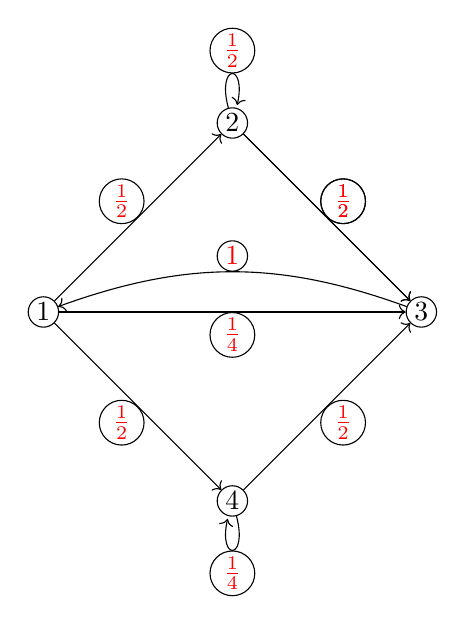
\begin{tikzpicture}[scale=1.2, every node/.style={draw, circle, inner sep=1pt}]
    \node (A) at (-2,0) {1};
    \node (B) at (0,2) {2};
    \node (C) at (2,0) {3};
    \node (D) at (0,-2) {4};

    \draw[->] (A) -- (B) node[midway, above left] {\textcolor{red}{$\frac{1}{2}$}};
    \draw[->, loop above] (B) edge node {\textcolor{red}{$\frac{1}{2}$}} (B);
    \draw[->] (B) -- (C) node[midway, above right] {\textcolor{red}{$\frac{1}{2}$}};
    \draw[->] (B) -- (C) node[midway, above right] {\textcolor{red}{$\frac{1}{2}$}};
    
    \draw[->] (A) -- (C) node[midway, below] {\textcolor{red}{$\frac{1}{4}$}};
    \draw[->, bend right=20] (C) to node[midway, above] {\textcolor{red}{$1$}} (A);
    \draw[->] (A) -- (D) node[midway, below left] {\textcolor{red}{$\frac{1}{2}$}};
    \draw[->, loop below] (D) edge node {\textcolor{red}{$\frac{1}{4}$}} (D);
    \draw[->] (D) -- (C) node[midway, below right] {\textcolor{red}{$\frac{1}{2}$}};
\end{tikzpicture}
\end{center}
$\{X_n\}$ is irreducible because for every $i,j \in S,$ there exists some $n$ such that $p^n(i,j) >0.$ To see this, consider that since $1\to 2 \to 3 \to 1,$ then $2\to 1$ and thus $3\leftrightarrow 1\leftrightarrow2.$ Similarly, $3\leftrightarrow1 \leftrightarrow4.$ By transitivity and symmetry, 
\[1 \leftrightarrow 2\leftrightarrow 3\leftrightarrow 4,\] and so $S$ itself is the only communication class.
    \end{solution}
    \item[(b)] Assume that the chain starts with \( X_0 = B \). What is the probability that \( X_3 = C \)?
\begin{solution}
    Using Wolfram, we see that 
    \[P^3 = 
\begin{pmatrix}
\frac{1}{2} & \frac{1}{4} & \frac{5}{16} & \frac{1}{4} \\
\frac{1}{4} & \frac{3}{8} & \frac{1}{4} & \frac{1}{4} \\
\frac{1}{4} & \frac{1}{4} & \frac{1}{2} & \frac{1}{4} \\
\frac{1}{4} & \frac{1}{4} & \frac{1}{2} & \frac{3}{8}
\end{pmatrix}
,\] and thus 
\[\boxed{p^3(C, B)} = \frac{1}{4}\]

\end{solution}
    \item[(c)] Under the same assumption as in the previous part, what is the probability that \( X_3 = C \), \( X_4 = A \), and \( X_6 = B \) all occur?
\begin{solution}
    \[P^4 = 
\begin{pmatrix}
\frac{5}{16} & \frac{3}{8} & \frac{3}{8} & \frac{3}{8} \\
\frac{1}{4} & \frac{5}{16} & \frac{3}{8} & \frac{1}{4} \\
\frac{1}{2} & \frac{1}{4} & \frac{5}{16} & \frac{1}{4} \\
\frac{1}{4} & \frac{1}{4} & \frac{3}{8} & \frac{5}{16}
\end{pmatrix}
\]
and so 
\[\boxed{p^4(A, B)} = \frac{3}{8}.\]
\[P^6(B, B) = \begin{pmatrix}
    \frac{29}{64} & \frac{23}{64} & \frac{7}{16} & \frac{23}{64}\\
    \frac{11}{32} & \frac{21}{64} & \frac{23}{64} & \frac{5}{16}\\
    \frac{3}{18} & \frac{11}{32} & \frac{29}{64} & \frac{11}{32}\\
    \frac{11}{32} &\frac{5}{16} & \frac{23}{64} & \frac{21}{64}
\end{pmatrix}\]
and so 
\[\boxed{p^6(B,B) = \frac{21}{64}}\]
\end{solution}
    \item[(d)] Compute the invariant probability vector for this Markov chain.
    \item[(e)] Let \( J_n \) denote the probability that at time \( n \) the system has been in state \( C \) exactly the same number of times it has been in state \( A \). Find
    \[
    \lim_{n \to \infty} J_n.
    \]
\end{enumerate}
\end{problem}

\end{document}